\section{Overall description}
%\writer{Thibaud}

This section describes the software and provides a brief explanation on how the system works.

\subsection{What are Petri nets?}

Petri nets are a graphical and mathematical modelling tool for describing concurrent and distributed systems. Some examples of their applications are workflow management, embedded systems or traffic control. The main advantages of Petri nets are their graphical notation, their simple semantics, and their rich theory for analysing their behaviour. However, using the graphical notation of Petri nets for understanding a complex system is quite hard, and thus a user-oriented visualization is required in a way that is understandable to users which are not necessarily familiar with Petri nets.


\begin{figure}[htp]
\begin{center}
  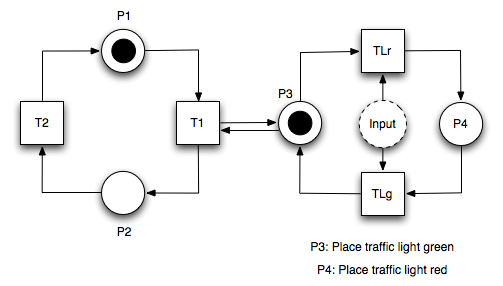
\includegraphics[width=0.8\textwidth]{image/petrinet_diagram_2.png}
  \caption{An example of a basic Petri net}
  \label{fig:petrinet}
\end{center}
\end{figure}

Figure \ref{fig:petrinet} presents an example of a basic Petri net. There are four different elements:

\begin{itemize}
\item Places: graphically represented by circles, represent conditions.
\item Transitions: graphically represented by squares, represent events.
\item Arcs: indicate which places are preconditions/postconditions for which transitions.
\item Tokens: graphically represented by the dots, represent the elements that are created and deleted in the Petri net along the places through the transitions.
\end{itemize}


As an example we can see Figure \ref{fig:petrinet} as a model for a railway with a traffic light. The token in Place P1 represents a train moving on a railway. When this train arrives to Place P1, the transition T1 will fire if there is also a token in Place P3. The only condition for a transition to be fired is that a token should be present on each of the incoming places of the transition.

In this scenario, the conditions are met, as the required token is in Place P3. The visualization of this scenario would be a traffic light with a green light. If instead Place P4 had a token on it and no token in P3, it would be a red light and the train would not be able to move. 

%If a user clicks on the Place I, it would generate a token that will turn the traffic light to green and thus the train will move.

With the aim of creating a visualization of the scenarios for the above Petri net model, an application tool is needed in order to allow the user to define where each of the elements are represented in the 3D world (geometry editor) as well as how these elements are represented (shape) and how they behave (animation). 

\subsection{Adding geometry to Petri nets}
The problem this project is tackled with is simple: We need a way to link the Petri net model to a 3D visualization, this is, to add extra information so that it can be visualized. Once a Petri net model is created and its real life design is well-designed in the user's mind, what we call a "Geometry" and "Appearance" are created. 

Once a Petri net model is created the user will be able to add a geometry and an appearance to it, in order to specify how the Petri net will look in the 3D visualization.

For this purpose, there is a need of a geometry editor which will be used to assign a two dimensional location to the elements defined in the Petri net, and of an appearance editor to take care of the shape of the elements.

\subsection{Adding appearance to Petri net objects}
\label{sec:appearance}

Once the geometry for the Petri net is defined, a shape for each object should be defined. For instance, places represent tracks and the 3D object or a shape and a texture should be linked to that place. The same applies to the transitions and tokens.

For this purpose, there is a need of an appearance editor which will be used to assign 3D visualization features to the elements defined in the Petri net.

The next step in visualizing Petri nets is add descriptive visuals. With the information provided by the Petri net, geometry and appearance as defined in the configuration file, the simulation is set up.

\subsection{Configuration}

Before running the simulation, a definition of how the models discussed above are connected is needed. This is done in the configuration step as well as the validity check for the Petri net's connections to the geometry. 

\subsection{Simulating Petri nets}

\begin{figure}[htp]
\begin{center}
	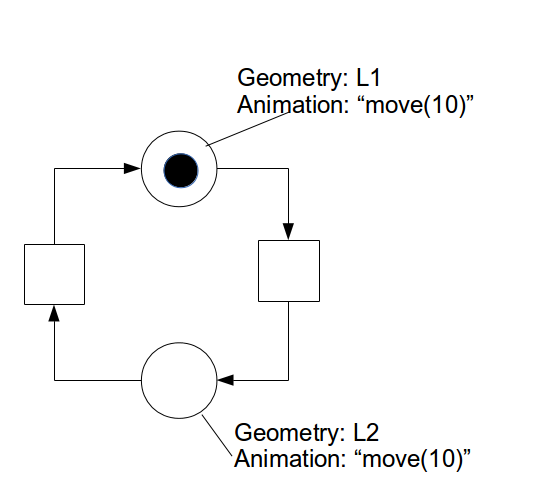
\includegraphics[width=\textwidth]{image/example_petrinet.png}
	\caption{A simple extended Petri net}
	\label{fig:example_petrinet}
\end{center}
\end{figure}

\begin{figure}[htp]
	\begin{center}
		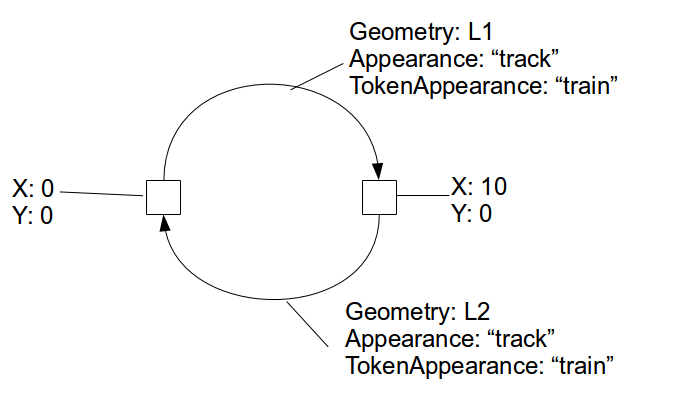
\includegraphics[width=\textwidth]{image/example_petrinet_geometry.png}
		\caption{A simple geometry}
		\label{fig:example_petrinet_geometry}
	\end{center}
\end{figure}


\begin{figure}[htp]
\begin{center}
  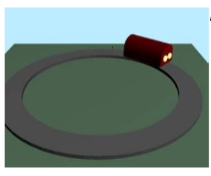
\includegraphics[width=0.4\textwidth]{image/3d.png}
  \caption{A simple 3D visualization}
  \label{fig:example_3d}
\end{center}
\end{figure}

%\begin{figure}[htp]
%\begin{center}
%  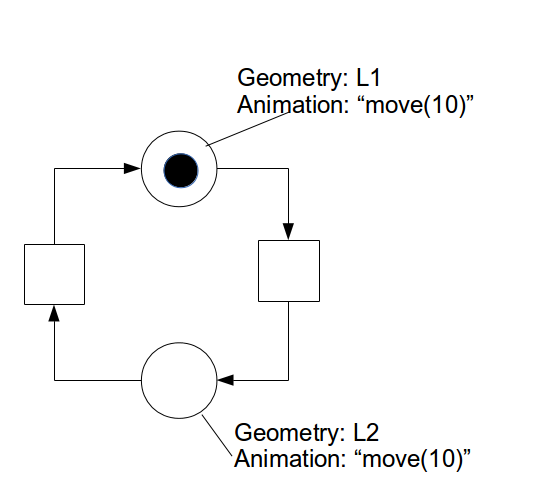
\includegraphics[width=0.4\textwidth]{image/example_petrinet.png}
%  \caption{A simple extended Petri net}
%  \label{fig:example_petrinet}
%\end{center}
%\end{figure}
%
%\begin{figure}[htp]
%\begin{center}
%  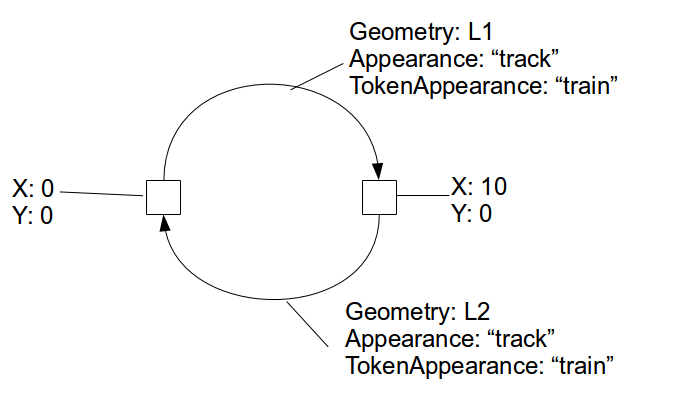
\includegraphics[width=0.4\textwidth]{image/example_petrinet_geometry.png}
%  \caption{A simple geometry}
%  \label{fig:example_petrinet_geometry}
%\end{center}
%\end{figure}

Using 3D models, textures and animations, the Petri net becomes easier to understand for the user. Continuing with the railway example, tokens become trains that move on tracks, which are places. As the tokens move from place to place, the train is animated in the 3D visualization along the tracks.

Figures \ref{fig:example_petrinet} and \ref{fig:example_petrinet_geometry} show how a simple 3D simulation of a train track and a train (Figure \ref{fig:example_3d}) is made out of Petri net model and a simple geometry. For example, in the Petri net model (Figure \ref{fig:example_petrinet}), Place P1 contains a geometry label that references its geometry location L1 in the geometry model (Figure \ref{fig:example_petrinet_geometry}).

\newpage

\subsection{General product overview \& use}

The overall description is a brief introduction to how our software is designed. For this purpose, it contains a description of the actors involved in its use, and also a description of how the software works. \newline

The following persons are all actors of our software:

\begin{itemize}
  \item Petri net engineer: An engineer whose role is to design and develop a Petri net which suits the company needs. \newline
  For instance, this could be an engineer working at a railway company and is in charge of modelling the railway system using Petri nets.
  \item End user: An actor to whom the Petri net 3D-Visualization would be presented, or an actor who is in charge of presenting the Petri net to another. \newline
	For instance, this could be a manager wanting to see what a Petri net represents. 
\end{itemize}

The software is built around three different concepts: 

\begin{itemize}
  \item Editors: A component responsible for handling the creation and design of one of our models. 
	\begin{itemize}
	 \item A Petri net editor to create a Petri net model.
	 \item A geometry editor to create and edit the geometry of the Petri net.
	 \item An appearance editor to set the appearance of the objects.
	 \item A configuration editor to configure the simulation.
	 \end{itemize}
	An editor is presented to the user as a GUI in an Eclipse window.
  \item Simulator: A simulator is, as its name says, a component capable of simulating a Petri net.
	The simulator is handling all the decisions regarding the Petri net and its behaviour. 
	It then communicates the decisions to a 3D Engine responsible for the visualization.
  \item 3D Engine: A 3D Engine is responsible for the visualization of a Petri net in three dimensions.
	It receives input from the Petri net simulator, and also communicates to the simulator when a user performs a certain type of action. \newline
	For example: the user clicks on a specific Place of the Petri net, this triggers a message from the 3D Engine to the Petri net simulator 
\end{itemize}
\newpage
Figure \ref{fig:system_diagram}. shows the different components of our system and their connections.

\begin{figure}[htp]
\begin{center}
  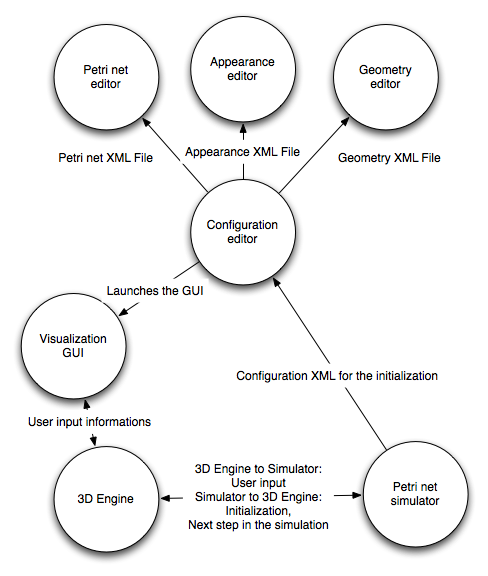
\includegraphics[width=0.6\textwidth]{image/system_design.png}
  \caption{System design}
  \label{fig:system_diagram}
\end{center}
\end{figure}

Moreover, this project also introduces new concepts related to Petri nets, because we are creating an extension to Petri nets.

Regarding \textbf{Petri nets}:
\begin{itemize}
  \item \textbf{Input Places}: An Input place is a place on which a user can create a token on Runtime, by interacting with the GUI in the form of a mouseclick. This token can then be used to trigger a transition for instance.
  \item \textbf{Geometry label}: A geometry label maps a place to a corresponding Geometry, defined later.
  A geometry label simply consists of an id.

  \item \textbf{Animation label}: An animation label describes the event happening on a place when a token is present.
Animation labels refer to either movement actions or trigger actions.\end{itemize}

A \textbf{Geometry} allows user to specify details about the 3D Space in which the Petri net is going to be rendered. It must present informations about the positions of the objects in the space but also informations about their looks.

\begin{itemize}
  \item \textbf{Appearance Label}: An appearance label maps a Geometry to a 3D model. One can find informations about appearances by reading further in this section.
  \item \textbf{A position}: The position of a geometry is deduced by the relative positions of the geometry objects in the editor. 
\end{itemize}

Finally, an \textbf{Appearance} file maps \textbf{Appearance Labels} to \textbf{3D models}.
To this end, each appearance label used by a Geometry corresponds to a file on the file system. The file is expected to be a 3D model.

\subsection{Basic functionality}


This software allows the engineers to create a Petri net 3D Visualization using a combination of the different editors built for this project.
The files created with each of the following editors are to be combined using the configuration editor: \newline
Petri net editor, Geometry editor, Appearance editor. 

In order to launch a simulation, an user should perform the following actions:

\begin{itemize}
  \item Create a Petri net model using the \textbf{Petri net Editor}. This editor is used to configure the Petri net.
  \item Create a Geometry model using the \textbf{Geometry editor}. This editor is used to map objects from the Petri net model to a corresponding Geometry. Geometries include informations about positions/paths in the 3D space. They may also keep a reference to an Appearance to define their texture and shape.
  \item Create an Appearance file using the \textbf{Appearance editor}. This editor is used to link appearance labels to 3D models. A label corresponds to a specific 3D model file. 
\end{itemize}

Once these three models have been created, the \textbf{Configuration editor} is used by the user to connect every model file previously created in order to be able to start a Simulation. 
To run the simulation, a specific "Run" button is added to the Configuration editor, which loads the Simulator.
\newline

The simulator then initializes the \textbf{3D Engine} with all the informations needed for the visualization. The 3D Engine then relies on the simulator to know which next move it should perform on the Petri net. \newline
To interact with the simulation, the user can either click or press certain keyboard buttons in the GUI for the visualization. \newline

\newpage
